\begin{figure}[h]
    \centering

    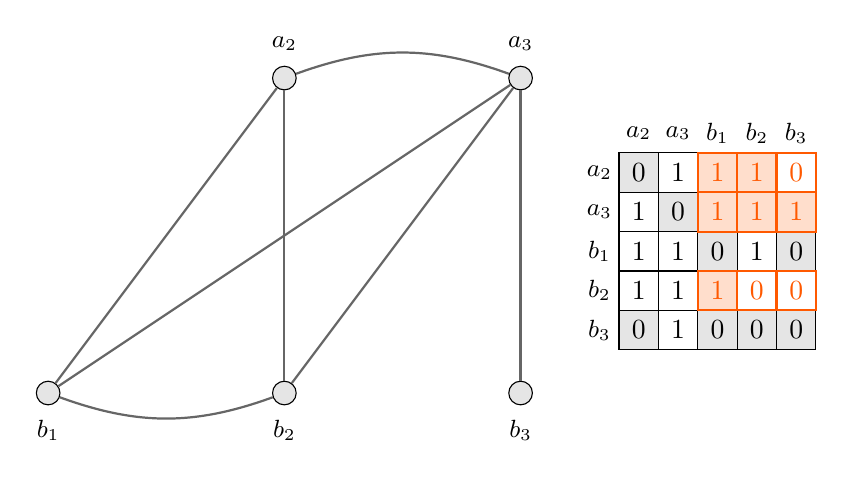
\begin{tikzpicture}[
        vertex/.style={circle, draw, fill=gray!20, minimum size=0.3 cm, inner sep=1pt},
        label_a/.style={above=2pt, font=\small},
        label_b/.style={below=2pt, font=\small},
        node distance=1.5cm,
        solid edge/.style={draw, thick, black!60},
        dashed edge/.style={draw, dashed, thick, black!40},
        matrix cell/.style={draw, minimum size=0.5 cm, inner sep=0pt},
        matrix label/.style={font=\small, anchor=center}
    ]
	\node[vertex] (b_1) at (3,-4) {};
	\node[vertex] (a_2) at (6,0) {};
	\node[vertex] (b_2) at (6,-4) {};
	\node[vertex] (a_3) at (9,0) {};
	\node[vertex] (b_3) at (9,-4) {};
	\draw[solid edge] (b_2) to [bend left=20] (b_1);
	\draw[solid edge] (a_2) -- (b_1);
	\draw[solid edge] (a_2) -- (b_2);
	\draw[solid edge] (a_3) -- (b_1);
	\draw[solid edge] (a_3) -- (b_2);
	\draw[solid edge] (a_3) -- (b_3);
	\draw[solid edge] (a_2) to [bend left=20] (a_3);
	\node[label_b] at (b_1.south) {$b_{1}$};
	\node[label_a] at (a_2.north) {$a_{2}$};
	\node[label_b] at (b_2.south) {$b_{2}$};
	\node[label_a] at (a_3.north) {$a_{3}$};
	\node[label_b] at (b_3.south) {$b_{3}$};

\begin{scope}[xshift=11 cm]
		\node[matrix cell, fill=gray!20] at (-0.5, -1.2) {0};
		\node[matrix cell] at (-0.5, -1.7) {1};
		\node[matrix cell] at (-0.5, -2.2) {1};
		\node[matrix cell] at (-0.5, -2.7) {1};
		\node[matrix cell, fill=gray!20] at (-0.5, -3.2) {0};
		\node[matrix cell] at (0.0, -1.2) {1};
		\node[matrix cell, fill=gray!20] at (0.0, -1.7) {0};
		\node[matrix cell] at (0.0, -2.2) {1};
		\node[matrix cell] at (0.0, -2.7) {1};
		\node[matrix cell] at (0.0, -3.2) {1};
		\node[matrix cell, fill=gray!20] at (0.5, -2.2) {0};
		\node[matrix cell, fill=gray!20] at (0.5, -3.2) {0};
		\node[matrix cell] at (1.0, -2.2) {1};
		\node[matrix cell, fill=gray!20] at (1.0, -3.2) {0};
		\node[matrix cell, fill=gray!20] at (1.5, -2.2) {0};
		\node[matrix cell, fill=gray!20] at (1.5, -3.2) {0};
		\node[matrix cell, thick, draw=orange!70!red, fill=orange!70!red!20, text=orange!70!red] at (0.5, -1.2) {1};
		\node[matrix cell, thick, draw=orange!70!red, fill=orange!70!red!20, text=orange!70!red] at (0.5, -1.7) {1};
		\node[matrix cell, thick, draw=orange!70!red, fill=orange!70!red!20, text=orange!70!red] at (0.5, -2.7) {1};
		\node[matrix cell, thick, draw=orange!70!red, fill=orange!70!red!20, text=orange!70!red] at (1.0, -1.2) {1};
		\node[matrix cell, thick, draw=orange!70!red, fill=orange!70!red!20, text=orange!70!red] at (1.0, -1.7) {1};
		\node[matrix cell, thick, draw=orange!70!red, text=orange!70!red] at (1.0, -2.7) {0};
		\node[matrix cell, thick, draw=orange!70!red, text=orange!70!red] at (1.5, -1.2) {0};
		\node[matrix cell, thick, draw=orange!70!red, fill=orange!70!red!20, text=orange!70!red] at (1.5, -1.7) {1};
		\node[matrix cell, thick, draw=orange!70!red, text=orange!70!red] at (1.5, -2.7) {0};
		\node[matrix label] at (-0.5, -0.7) {${a_2}$};
		\node[matrix label] at (-1, -1.2) {${a_2}$};
		\node[matrix label] at (0.0, -0.7) {${a_3}$};
		\node[matrix label] at (-1, -1.7) {${a_3}$};
		\node[matrix label] at (0.5, -0.7) {${b_1}$};
		\node[matrix label] at (-1, -2.2) {${b_1}$};
		\node[matrix label] at (1.0, -0.7) {${b_2}$};
		\node[matrix label] at (-1, -2.7) {${b_2}$};
		\node[matrix label] at (1.5, -0.7) {${b_3}$};
		\node[matrix label] at (-1, -3.2) {${b_3}$};
    \end{scope}

    \end{tikzpicture}
    \caption{\emph{On the left}, an example of a graph smaller than a $3\times3$ half-graph thatfor which no induced copies can be found in a $3$-stable graph. It is basically a $3\times3$ half-graph in which $a_1$ and $b_2$ are the same vertex, and an edge isadded between $a_2$ and $a_3$.
\emph{On the right}, the corresponding adjacency matrix.Orange cells highlight edges relative to the $3$-order structure}
    \label{fig:other_k-order}
\end{figure}
